\documentclass[sigplan,10pt,review,anonymous]{acmart}

% Packages {{{
\usepackage{amsmath}
\usepackage{amssymb}
\usepackage{tikz}
\usetikzlibrary{calc}
\usetikzlibrary{graphs}
\usetikzlibrary{cd}
\usepackage{bussproofs}
\usepackage{stmaryrd}
% }}}

% Macros {{{

\newcommand{\kw}[1]{\ensuremath{ \textsf{#1} }}
\newcommand{\ifr}[1]{\ [{#1}]\ }
\newcommand{\ifrw}[2]{\ [{#1}]_{#2}\ }
\newcommand{\alt}{\ |\ }

\newcommand{\EC}{\kw{C}}
\newcommand{\simrel}{\kw{simrel}}

% Moves
\newcommand{\mcall}[3]{\kw{#1}({#2})@{#3}}
\newcommand{\pcall}[3]{%
  \underline{\mcall{#1}{#2}{#3}}%
}
\newcommand{\mret}[2]{{#1}@{#2}}
\newcommand{\pret}[2]{%
  \underline{\mret{#1}{#2}}%
}
\newcommand{\mretx}[3]{{#1}@{#2}/{#3}}
\newcommand{\pretx}[3]{%
  \underline{\mretx{#1}{#2}{#3}}%
}

% Pointers for justified sequences %{{{

% Parameters
\newcommand{\pshift}{1.6ex}
\newcommand{\pcdist}{2.5}
\newcommand{\pcangle}{60}

% Pointer hook
\newcommand{\ph}[1]{%
  \tikz[remember picture]{\coordinate (#1);}}

% Pointer to
\newcommand{\pt}[1]{%
  \rule{0pt}{1.4em}%
  \tikz[remember picture, overlay]{
    \draw[->]
      let \p{dest} = (#1),
          \n1 = {ln(veclen(\x{dest}, \y{dest}) + 1)},
          \p1 = ($(0,0)+(0,\pshift)$),
          \p4 = ($(#1)+(0,\pshift)$),
          \p2 = ($(\p1)!\n1*\pcdist!-\pcangle:(\p4)$),
          \p3 = ($(\p4)!\n1*\pcdist!+\pcangle:(\p1)$) in
        (\p1) .. controls (\p2) and (\p3) .. (\p4);}}

%}}}

% }}}

% Various parameters {{{
\bibliographystyle{ACM-Reference-Format}
\citestyle{acmnumeric}
%}}}

\begin{document}

\title[%
  A Compiler Suitable for End-to-End Verification%
]{%
  A Certified Compiler Suitable for End-to-End Verification of Computer Systems%
}

\author{J\'er\'emie Koenig}
\affiliation{
  \department{Computer Science}
  \institution{Yale University}
}
\email{jeremie.koenig@yale.edu}

\begin{abstract} %{{{
We identify six requirements
for a foundational theory of components
which can support the grand challenge of
end-to-end specification and verification of large-scale systems:
expressivity,
compositionality,
openness,
and the ability to account for
refinement,
abstraction,
and resources.

Existing research
in the field of programming language semantics
has tackled various combinations of these requirements
in a variety of contexts,
but a satisfactory theory addressing all six has yet to emerge.
In particular,
while traditional work on game semantics
has successfully addressed the first three,
work in this area does not typically focus
on refinement, abstraction and resources as central concepts.
Conversely,
work in the latter areas
often remains very specific (lacking expressivity),
and typically fails to account for open systems.

We conjecture that
a successful synthesis of these disparate strands of research
can yield the theory we seek.
[As an illustration,
we work out how these ideas play out in the context of compilers,
and show they can be applied
to solve the open problem of compositional certified compilation.]
\end{abstract}
%}}}

\maketitle

\section{Introduction} %{{{

[Say a thing or two about formal methods and
the goal of end-to-end verification of computer systems.
Mention reliability of the information infrastructure,
cyber-physical systems, etc.]

[Vision of a compositional theory of systems
supporting large-scale reasoning:
about the global information infrastructure from the transitors,
about the likelihood of your self-driving car getting in an accident
from the laws of physics, etc.]

The contribution of PL/CS to the general theory of systems
must be \_ [a logic of models, or whatever].

Challenges:
\begin{enumerate}
\item Expressivity.
  [Need not be achieved all at once,
  if we can embed the semantic domain used to analyse a system
  into a broader one.
  The bar should be,
  our formalism should be rich enough to account for
  the full range of possible interaction of a system with its environment
  in the real world.
  Then there should be a way to embed in the formalism
  used to analyze / build any larger system of which it is a component.
  We demonstrate this when we build our richer semantics of Compcert in Sec~4
  and embed our minimalistic one from Sec~3.]
\item Compositionality.
  [Complex systems can only be understood
  as the relationship of simpler components,
  which can be reasoned about in isolation.]
\item Open systems.
  [Compositionality should work from the bottom up, not top down.
  Components should not be understood as fragments of a fixed whole.
  There is no whole system.
  Every system is a component.
  \emph{But},
  it may be reasonable to partially close a subsystem
  after we built it up from components,
  as long as the resulting one
  is still able to interact with its environment]
\item Abstraction.
  [Reductionism is shit.
  You can't \emph{understand} a book
  as a collection of atoms of ink, paper and glue.
  Let alone how that relates to the corresponding e-book.
  Let alone its place within a genre of literature.
  Every level of abstraction exists in its own right.
  Its nature cannot be explained by a particular realization.
  The relation between them ]
\item Refinement.
  [The role of a component is realized in a specific way.
  We don't want to sweat the details when looking at the big picture.]
\item Resources.
  [The role of a component is realized in an imperfect way.
  An ideal, infinite model only exists in the real world
  as a series of finite approximations;
  resource limitations introduce a discontinuity.
  Abstractions break down beyond certain threshold:
  we run out of stack space,
  insufficient network capacity introduces congestion,
  a heap becomes too fragmented to satisfy
  requests for a contiguous block of memory.

  A satisfactory treatment of resources
  allows us to caracterize the range of conditions
  under which refinement and abstraction hold,
\end{enumerate}

Programming language theory [has experience with all of these, though not all at once]
Hence has a key contribution to bring to a general systems theory,
if we can gather the strands into a coherent whole.

In the context of the theory programming languages,
[enumerate things that have tackled combinations of these
challenges:
subtyping -> refinement;
traditional game semantics -> expressivity, compositionality, open systems;
interface automata -> compositionality, $\approx$ open systems, refinement;
certikos -> abstraction, refinement;
lax modality -> compositionality, resources;
logical relations -> abstraction and refinement (sometimes), compositionality;
...]

Research program:
gather these threads to develop the mathematical foundations
for a theory of systems
that can support end-to-end verification of computer systems
and more.

In this paper:
sketch something for challenges 2-5
out of (traditional game semantics + interface automata + abstraction layers).
Illustrate how these ideas play out in the context of compilers,
and apply them to solve the open problem of
compositional certified compilation.

\subsection{Compilers} %{{{

Compilers play an essential role in the construction
of present-day computer systems.

[Explain what a compiler is.
Central to the task of building computer systems.]

Given the many complicating factors,
it's no surprise that compositional certified compilation
remains open problem.
[Give a table of exisiting work and which aspects they address,
and review in the text explaining why they fail/succeed each aspect]

Ex.: original compcert uses relatively expressive model
(event traces are fairly general),
and has a notion of refinement (inclusion of sets of behaviors, Vundef),
but not compositional (whole program),
not that open (it's unclear how to connect all kinds of interesting things),
no abstraction (behavior of source and target expressed in same model),
no account of resources (infinite stack at Asm).

Various works seek to extend to support some of these things:
CompCompCert, separate compcert, CompCertX, Qompcert

%}}}

\subsection{Challenges} %{{{

[Compositional Compcert still an open problem]

[Compositional system model even more:
mention that Compcert's model of the userspace is very naive;
impossible to encode a specification such as POSIX
as external function semantics]

%}}}

\subsection{Contributions} %{{{

This works aims to make a contribution
towards the grand challenge of end-to-end verification
of large-scale systems,
by advancing a conceptual framework
[for understanding suitability / guiding design
of theories and components that may participate.]

Specifically,
we identify six principles [...]
Give a clear ``test'' for each.
Can guide design.

To substantiate this claim,
we apply our analytical framework to the problem of certified compilation:
\begin{itemize}
\item analyze previous work in pl semantics and certified compilation
  in this framework to assess and explain the strenghts and weaknesses of each
  [sec. 12 Related Work]
\item show [in sec. 3 Semantics with External Calls]
  how these ideas yield a natural solution
  when applied to the open problem of compositional compilation
\item formulate new challenge / next step:
  that of a compiler which can be used as a component
  for end-to-end verification;
\item In Sec.~4 [richer semantics],
  show that our semantic model can be made more expressive
  in a way that our compiler remains correct in that setting;
\item In Sec.~5 [applications],
  illustrate with some applications
  the ways in which our compiler can be connected
  to a larger system
\item Assess the remaining gap between our compiler
  and our new challenge (concurrency, resources),
  and apply our analytical framework to suggest
  what a solution might look like.
\end{itemize}

[Basic claim: the answer to compositional verification
is an undestanding of abstraction and refinement in the context of games.]
The present work applies this analysis to
solve the open problem of certified compositional compilation of low-level languages
plus an understanding of refinement and abstraction in that context.]

%}}}

\subsection{Limitations} %{{{

No concurrency
(not expressive enough:
accesses to memory between external calls are not observable
--- this being said existing work on Concurrent CertiKOS shows
it may be possible to map our model in a more general one),
no good story for resources.

In Sec.~N [Future Work] [spell out some leads to fill these gaps.]

%}}}

%}}}

\section{Certified Compilation} %{{{

Formally,
a programming language $L$ is understood as
a set of programs $p$
which are assigned a meaning $\llbracket p \rrbracket$
in a semantic domain $\mathbb{D}$.
We call \emph{programs} or \emph{modules} the elements of $L$,
preferring the latter when the language supports
a notion of composition where modules are expected to
interact and be linked with other modules of the same kind.
We call \emph{behaviors} or \emph{specifications}
the elements of $\mathbb{D}$,
preferring the latter whan the semantic domain supports
a notion of refinement and the specification under consideration
may be refined by more specific behaviors.

In this context,
a compiler can be understood as a function
$C : L_s \rightarrow L_t$
which transforms a source program $p \in L_s$
into a target program $C(p) \in L_t$.
When the two languages are interpreted into
a common semantic domain,
the correctness of the compiler can simply be stated as:
\[ \llbracket C(p) \rrbracket_t =
    \llbracket p \rrbracket_s \]
That is,
the source and target programs have the same behavior.
However,
to take into account the complexity of real-world languages and compilers,
we must generalize this approach.

\subsection{Expressivity} %{{{

Although communication model between program
and the underlying system is simple and uniform
(system calls / external function invocation),
this protocol is general enough that
when we link with the outside world,
the source/target machine models are enough to
implement all kinds of stuff:
network services, GUIs, drivers, control software,
operating systems, distributed computations, \ldots
The same compiler is used in all of these contexts.

%}}}

\subsection{Compositionality} %{{{

[Large programs are split into compilation units,
which are compiled independently,
then linked to produce the final artefact.]

%}}}

\subsection{Abstraction} %{{{

The assumption that the source and target programs
can be naturally assigned meanings in the same semantic domain
is reasonable for some individual compiler passes and optimizations
where the source and target languages are fairly similar.
It can also hold when observable behaviors are simple:
if we are only interested in whether the program terminates
and produces a given result,
then the corresponding notion of behavior
can be fairly language-independent.
However,
in most practical cases we are interested in
the program's interaction with its environment
as well as its ultimate outcome,
and this interaction is often understood very differently
in the context of the source and target languages.

For instance,
in the C programming language
the memory is understood in terms of independent objects.
Each object corresponds to a variable declared in the program,
or to a chunck of heap-allocated memory.
A function call is performed by allocating new objects
corresponding to the callee's arguments and local variables,
then initializing the callee's arguments
using the values provided by the caller.
By contrast,
an assembly program
operates in a single address space,
and the memory is essentially seen as a single array of bytes.
Likewise,
the very notion of a function call in assembly
is largely conventional as opposed to a primitive notion,
and their mechanics are understood in very different terms.

Consequently,
semantic domains that naturally reflect and accurately account
for module interaction in C and assembly will necessarily be distinct.
This underscore importance of \emph{abstraction}:
C compilers operate in the context of a given \emph{calling convention},
which establishes a relationship between the behaviors of C modules
and that of assembly modules.
This calling convention can be modelled as a function
$\mathbb{C} : \mathbb{D}_s \rightarrow \mathbb{D}_t$,
which is in some sense the semantic counterpart to the compiler $C$.
Our correctness criterion becomes:
\[ \llbracket C(p) \rrbracket_t =
    \mathbb{C}(\llbracket p \rrbracket_s) \]

[Compcert goes to great length to ensure $\mathbb{D}_s = \mathbb{D}_t$,
defining unified memory model etc.
Much compositional Compcert works keeps with this approach
but this creates problems.
In fact, even when $\mathbb{D}_s = \mathbb{D}_t$ formally,
the source and target behaviors may be distinct
and it can be important/useful to define
$\mathbb{C} : \mathbb{D} \rightarrow \mathbb{D}$.
In Sec.~N we show how taking abstraction seriously
solves the extcall\_args problem.]

%}}}

\subsection{Refinement} %{{{

In and of itself,
abstraction is insufficient to reflect
the relationship between the behaviors of C and assembly modules.
This is because there is more than one way to realize
a given C call at the level of assembly.
For instance,
a typical calling convention specifies a classification of machine registers
into \emph{callee-save} registers,
which are guaranteed to be left unchanged by the function being invoked,
and \emph{caller-save} registers,
which the function being invoked may modify at will.
Therefore,
two assembly functions may realize the same C behavior
but be observationally distinct at the level of assembly
if they return with different values in the callee-save registers.

To account for this situation,
the target semantic domain $\mathbb{D}_t$
should contain specifications
allowing a range of possible behaviors,
and be equipped with a notion of refinement
in the form of a preorder $\sqsubseteq$.
The target behavior $\mathbb{C}(\sigma_s)$
corresponding to the source behavior $\sigma_s$
can then be broad enough to state,
for instance,
that the callee-save registers
may contain any value after a function
specified in $\sigma_s$ returns.
The behaviors of target programs
which leave specific values in these registers
but otherwise agree with $\mathbb{C}(\sigma_s)$
will be considered valid implementations.
Taking this into account,
the correctness statement becomes:
\[ \llbracket C(p) \rrbracket_t \sqsubseteq
    \mathbb{C}(\llbracket p \rrbracket_s) \]

Note that while abstraction and refinement are distinct concepts,
it can sometimes be advantageous to unify them
in the form of a single, heterogenous relation
${\sqsubseteq_\mathbb{C}} = {\sqsubseteq} \circ {\mathbb{C}}$.
[Reference popl15's abstraction relations]
[Forward reference to where we do that in this work].
[Explain that confusing the two root of some limitation
in existing work].

[Comment on induced equivalence relation?]

[Role of refinement/abstraction in permitting optimizations?]

%}}}

\subsection{Open systems} %{{{

subsets of behaviors is not good enough,
we need to take distinction between system and environment seriously.
-> this is how we define a notion of refinement in Sec.~3
that solves some of the issues

Discuss contextual refinement,
which is not enough \emph{a priori}, and \emph{practically},
because we don't want to limit ourselves to a set of systems we're gonna connect with.
In this way logical relations are more fundamental,
and then the derived contextual refinement is useful
in the special case where the system we embed our program in
is itself a program written in the same language.
But also contextual refinement might be enough
if the interaction of all the environments we would ever want to connect with
can be "coobservationally equivalent" to a context in our set
from the point of view of the program (aka oracle).

[The compilation of one module
makes no assumption as to what other modules are going to be using it.
Library. Contextual refinement.
The operating system can do all kinds of crazy stuff to you:
signals, memory-mapped I/O, fork, etc,
but the compiler remains correct in the context of that intereference.

Specs need to be able to express constraints on the environment.]

%}}}

\subsection{Resources} %{{{

[The source model is usually much more idealized than target.
Example: infinite stack vs. finite address space.]

%}}}

\subsection{Putting it all together} %{{{

%}}}

\subsection{The Compcert Certified Compiler} %{{{

\paragraph{Semantic Domains}
\paragraph{Transition Systems}
\paragraph{Memory Model}
\paragraph{External Calls}
\paragraph{Correctness}

%}}}

%}}}

\section{Per-Function Semantics with External Calls} %{{{

\subsection{Semantic Domain}

In order to make Compcert truly ...

\begin{align*}
  e \in \mathbb{E}_\kw{C} &::=
    \cdots | \kw{extcall}[f, \vec{v}, m, \mathbb{b}] \\
  \sigma \in \mathbb{D}_\kw{C} &=
    \kw{ident} \rightarrow \mathbb{E}_\kw{C}
\end{align*}

\subsection{Transition Systems}
\subsection{Compiler Correctness}

%}}}

\section{A Richer Semantic Domain} %{{{

\subsection{Games}
\subsection{Strategies}


%}}}

\section{Applications} %{{{

\subsection{Non-Local Jumps}
\subsection{Context Switching}
\subsection{Thread library}
\subsection{File-System Interaction}

%}}}

\section{Future Work} %{{{

\subsection{Signals}
\subsection{Concurrency}
\subsection{Relaxed Memory Models}
\subsection{Abstraction of Values} %parametricity? can use pointers + empty mem block?

%}}}

\section{Related Work}
\section{Conclusion}


\bibliography{lwcc}

\appendix %{{{

\section*{Old abstract}

A simple game semantics based on a form of standard pointer games
is defined for the Clight and Asm languages of Compcert,
along with appropriate notions of simulation and linking.
The correctness theorem of CompCertX \citep{popl15}
is generalized to that setting,
turning it into a compositional compiler
similar to Compositional Compcert \citep{compcomp}.

As a technical device,
we introduce a family of Kripke logical relations for Compcert
which generalize the notions of memory extension and injection
around which Compcert's simulation relations are constructed,
and can also encode some invariants used in Compcert.
In this setting,
the constraints that Compcert imposes on the semantics of external functions,
as well as many properties of Clight and Asm,
find a natural expression as a form of relational parametricity.

Our game semantics is constructed from the original
small-step semantics of Compcert,
which is probed to reconstitute the interaction of the program:
calls from the program into the environment and
the program's eventual outcome
are recorded as moves of the program,
whereas the initial call into the program and
results from external functions
are recorded as moves of the environment.
Each move is equipped with a pointer to an earlier move,
which for function calls designates the parent activation,
and for return moves designates the function call being answered.

Compcert Kripke logical relations are deployed in this context
to define a notion of simulation between strategies.
Rather than a simple temporal succession of moves,
the Kripke modality used in these simulations
follows the activation tree structure
encoded by the moves' pointers.
By leveraging this structure in our simulations
we can avoid some of the complications
that arise in existing work on compositional compilation.

\section{Introduction} %{{{

Problem:
compositional compilation.
System code:
link compiled C code with less well-behaved assembly code,
interact and compose with components of different types
(hardware, networks, etc.).

Existing things limited:
Compositional Compcert only works with one type of games
and proof requires modifying Compcert pretty deep,
new techniques and lots of effort to implement,
hence hard to integrate to mainstream Compcert.

Our semantic algebra less ad-hoc and follows HO games.

Our technique allow us to prove a linking theorem for Compcert
without modifying the original proofs:
leverage the external functions interface as a hook
through which we can expose Compcert to its environment in a controlled way.
Bridge the gap with some game-theoretic algebra.

KLR/parametricity understanding of Compcert languages provides
uniform easy natural definition of refinement
that works well with the existing code,
shed new light on the construction of Compcert.

Some context we can bring up:
separate compilation,
compositional compilation (definition, see ZS whiteboard; compositional compcert),
compositional verification,
models of and linking with non-software components
(devices, network systems, physical world, etc.)

\subsection{Compositional compilation}

To have a compositional compiler we must define:
\begin{itemize}
\item a semantic domain $\mathbb{D}$;
\item operators $\llbracket - \rrbracket_\kw{s}$, $\llbracket - \rrbracket_\kw{t}$
  associating to each source and target program a semantics in $\mathbb{D}$;
\item a linking operator $\bowtie \: : \mathbb{D} \times \mathbb{D} \rightarrow \mathbb{D}$;
\item a refinement relation ${\sqsubseteq} \subseteq \mathbb{D} \times \mathbb{D}$.
\end{itemize}
The semantics should be sound in the sense that
two programs with the same denotation should be observationally equivalent.
The refinement relation should be a partial order.
The linking operator should be associative and commutative,
and should satisfy:
\[
  \AxiomC{$\sigma_1 \sqsubseteq \sigma_1'$}
  \AxiomC{$\sigma_2 \sqsubseteq \sigma_2'$}
  \BinaryInfC{$\sigma_1 \bowtie \sigma_2 \sqsubseteq \sigma_1' \bowtie \sigma_2'$}
  \DisplayProof
\]
In addition,
we expect the following theorem to hold
for the languages under consideration,
which relates the semantic linking operator to
the syntactic composition of modules:
\[
  \llbracket M_1 + M_2 \rrbracket \equiv
  \llbracket M_1 \rrbracket \bowtie \llbracket M_2 \rrbracket
\]
Then a compiler $\mathcal{C}$ is correct if
for all source programs $p$:
\[
  \llbracket \mathcal{C}(p) \rrbracket_\kw{t} \sqsubseteq
  \llbracket p \rrbracket_\kw{s}
\]

\subsection{Contributions}

A new approach for building compositional certified compilers:
\begin{itemize}
\item (first applied?) mechanized formalisation of pointer games
\item Compcert KLRs
\item extend KLR to strategies, game-theoretic simulations
\item a game semantics for the Clight and Asm languages of Compcert
\item game-theoretic characterization of CompCertX's correctness theorem, from which we derive
\item a \emph{semantic} contextual refinement property
\end{itemize}

%}}}

\section{Kripke logical relations for Compcert} %{{{

%XXX: how does this relate to
%the intrinsic preorder in 3.5 of [Abramsky \emph{Game Semantics}]?
%Sound/complete reasoning principle?

\subsection{Logical relations} %{{{

In the broadest sense,
logical relations are structure-preserving relations,
in the same way that homomorphisms are structure-preserving maps
\citep{lrp}.
Logical relations can be of any arity,
but in the present work
we restrict our attention to
binary logical relations.
Given a structure $\mathcal{S}$
involving a number of operations over a carrier set,
a \emph{logical relation}
between two instances $S_1, S_2$ of $\mathcal{S}$
will be a relation $R \subseteq |S_1| \times |S_2|$
between their carrier sets,
such that the operations of $\mathcal{S}$
take related arguments to related results.
We write $R : \mathcal{R}(S_1, S_2)$.

\begin{example}[Logical relation of monoids]
\label{ex:monoid}
A \emph{monoid} is a set $A$ equipped with
an associative binary operation $\cdot$ and
an identity element $\epsilon$.
A \emph{logical relation of monoids} between
a monoid $\langle A, \cdot_A, \epsilon_A \rangle$ and
a monoid $\langle B, \cdot_B, \epsilon_B \rangle$
is a relation $R \subseteq A \times B$
such that:
\begin{gather*}
u \ifr{R} u' \wedge v \ifr{R} v' \Rightarrow u \cdot_A v \ifr{R} u' \cdot_B v' \\
\epsilon_A \ifr{R} \epsilon_B
\end{gather*}
[Possible example: some ``coded message'' relation,
where sequences on the left correspond to sequences on the right,
not possible with monoid homomorphisms.]
\end{example}

Logical relations between multisorted structures
will include one relation for each sort,
between the corresponding carrier sets.
In the case of structures which include type operators,
we can associate to each base type $A$
a relation over its carrier set $\llbracket A \rrbracket$,
and to each type operator $T(A_1, \ldots, A_n)$
a corresponding \emph{relator},
which given relations $R_1, \ldots, R_n$ over
the carrier sets $\llbracket A_1 \rrbracket, \ldots, \llbracket A_n \rrbracket$
will construct a relation $T(R_1, \ldots, R_n)$
over $\llbracket T(A_1, \ldots, A_n) \rrbracket$.

Relators for some common constructions are shown in Fig.~\ref{fig:relators}.
Note that the first requirement given in Ex.~\ref{ex:monoid}
can be expressed as:
\[
  \cdot_A \ifr{R \times R \rightarrow R} \cdot_B
\]

\begin{figure}
  \begin{align*}
    x \ifr{R_1 \times R_2} y \ \Leftrightarrow\  &
      \pi_1(x) \ifr{R_1} \pi_1(y) \wedge
      \pi_2(x) \ifr{R_2} \pi_2(y) \\
    x \ifr{R_1 + R_2} y \ \Leftrightarrow\  &
      (\exists \, x_1 \, y_1 \,.\,
        x_1 \ifr{R_1} y_1 \wedge
        x = i_1(x_1) \wedge
        y = i_1(y_1)) \vee \\ &
      (\exists \, x_2 \, y_2 \,.\,
        x_2 \ifr{R_2} y_2 \wedge
        x = i_2(x_2) \wedge
        y = i_2(y_2)) \\
    f \ifr{R_1 \rightarrow R_2} g \ \Leftrightarrow\  &
      \forall \, x \, y \,.\,
        x \ifr{R_1} y \Rightarrow
        f(x) \ifr{R_2} g(y) \\
    A \ifr{\mathcal{P}^+(R)} B \ \Leftrightarrow\  &
      \forall \, x \in A \,.\,
      \exists \, y \in B \,.\,
      x \ifr{R} y \\
    A \ifr{\mathcal{P}^-(R)} B \ \Leftrightarrow\  &
      \forall \, y \in B \,.\,
      \exists \, x \in A \,.\,
      x \ifr{R} y
  \end{align*}
  \caption{A selection of relators}
  \label{fig:relators}
\end{figure}

[Explain use in PL theory better]

%}}}

\subsection{Kripke logical relations} %{{{

For stateful languages,
which terms should be related
will often depend on the current state of the store.
This motivated the introduction of Kripke logical relations.
[Some more background and references here.]

\begin{definition}[Kripke logical relation]
A \emph{Kripke frame} is a structure $\langle W, \leadsto \rangle$, where
$W$ is a set of \emph{possible worlds}, and
$\leadsto$ is an \emph{accessibility relation}
between the sets $W + \{\star\}$ and $W$.
Then a \emph{Kripke logical relation} is
a $W$-indexed family of logical relations $(R_w)_{w \in W}$.
\end{definition}

We write $R : \mathcal{R}_W(S_1, S_2)$
for a Kripke logical relation between structures $S_1$ and $S_2$.
Note that our Kripke frames
include a set of \emph{initial worlds}
$W* = \{ w \in W \ |\  \star \leadsto w \}$.
This will be useful when interpreting Kripke logical relations
as regular logical relations
by interpreting $\star$ as the ``current'' or ``actual'' world.
In the context of our game semantics,
the peculiar form of the definition
also facilitates the correspondance with
our arenas' enabling relations,
as defined in Sec.~\ref{sec:games}.

\paragraph{Relators}

For a given Kripke frame $\langle W, \leadsto \rangle$,
a logical relation $R : \mathcal{R}(A, B)$
can be promoted to a $W$-indexed Kripke logical relation $\lceil R \rceil$
which ignores the index, so that $\lceil R \rceil_w = R$.
Likewise,
a relator
  $F : \mathcal{R}(A_1, B_1) \,\times\,\cdots\,\times\,\mathcal{R}(A_n, B_n) \rightarrow \mathcal{R}(A, B)$
can be promoted to its Kripke version
by pointwise extension over the set of possible worlds:
\begin{gather*}
  \lceil F \rceil : \mathcal{R}_W(A_1, B_1) \times \cdots \times \mathcal{R}_W(A_n, B_n) \rightarrow \mathcal{R}_W(A, B) \\
  \lceil F \rceil (R_1, \ldots, R_n)_w = F(R_{1,w}, \ldots, R_{n,w})
\end{gather*}
In addition,
$\Box, \Diamond : \mathcal{R}_W(A,B) \rightarrow \mathcal{R}_W(A,B)$
are the Kripke relators defined by:
\begin{align*}
  x \ifr{(\Box R)_w} y &\Leftrightarrow
    \forall w' \,.\, w \leadsto w' \rightarrow x \ifr{R_w} y \\
  x \ifr{(\Diamond R)_w} y &\Leftrightarrow
    \exists w' \,.\, w \leadsto w' \wedge x \ifr{R_w} y
\end{align*}
We also define
$\Box, \Diamond : \mathcal{R}_W(A,B) \rightarrow \mathcal{R}(A,B)$
which turn a Kripke logical relation $R$
into (regular) logical relations as follows:
\begin{align*}
  x \ifr{\Box R} y &\Leftrightarrow
    \forall w' \,.\, \star \leadsto w' \rightarrow x \ifr{R_w} y \\
  x \ifr{\Diamond R} y &\Leftrightarrow
    \exists w' \,.\, \star \leadsto w' \wedge x \ifr{R_w} y
\end{align*}

\begin{example}[Simulation diagram]
\label{ex:sim}
Consider a Kripke logical relation of sets $R : \mathcal{R}_W(A, B)$,
and two transition relations $\alpha : A \rightarrow \mathcal{P}(A)$
and $\beta : B \rightarrow \mathcal{P}(B)$.
The simulation diagram:
\[
  \begin{tikzcd}
    s_1 \arrow[r, "\alpha"]
        \arrow[d, dash, "R_w"'] &
    s_1' \arrow[d, dotted, dash, "R_{w'} \quad (w \leadsto w')"] \\
    s_2 \arrow[r, dotted, "\beta"] &
    s_2'
  \end{tikzcd}
\]
can be written as:
\[
  \alpha \ifr{\Box (R \rightarrow \mathcal{P}^+(\Diamond R))} \beta \,.
\]
\end{example}

Likewise,
the simulation relations used by Compcert can be understood
as Kripke logical relations.
For instance,
the basic types used to defined the semantics of Compcert languages
are equipped with a notion of \emph{memory injection}
(a special case of Kripke logical relation).
Operations over these types
satisfy properties similar to the simulation diagram in Ex.~\ref{ex:sim}.
These basic operations are composed
to obtain operational semantics
which themselves
satisfy such properties.

This approach can be generalized:
In the remainder of this section,
we define a notion of \emph{Compcert KLR},
which admits Compcert's injections and extensions
as particular instances,
but makes it possible to encode
a broader range of properties.

%}}}

\subsection{Compcert KLRs} %{{{

\begin{figure} % fig:cklr (Compcert KLRs) {{{
  Values ($R^\kw{val}$)
  \vspace{1em}
  \[
    \begin{array}{r@{\,}l@{\hspace{3em}}c}
      v : \kw{val} ::= &
        \kw{Vundef} &
        \kw{Vundef} \ifr{\Box R^\kw{val}} \kw{Vundef} \\
      \alt &
        \kw{Vint}(n) &
        \kw{Vint} \ifr{(=) \rightarrow \Box R^\kw{val}} \kw{Vint} \\
      \alt &
        \kw{Vlong}(n) &
        \kw{Vlong} \ifr{(=) \rightarrow \Box R^\kw{val}} \kw{Vlong} \\
      \alt &
        \kw{Vfloat}(x) &
        \kw{Vfloat} \ifr{(=) \rightarrow \Box R^\kw{val}} \kw{Vfloat} \\
      \alt &
        \kw{Vsingle}(x) &
        \kw{Vsingle} \ifr{(=) \rightarrow \Box R^\kw{val}} \kw{Vsingle} \\
      \alt &
        \kw{Vptr}(p) &
        \kw{Vptr} \ifr{\Box (R^\kw{ptr} \rightarrow R^\kw{val})} \kw{Vptr}
    \end{array}
  \]
  \vspace{1em}
  \[
    \AxiomC{$w \leadsto w'$}
    \UnaryInfC{$R^\kw{val}_w \subseteq R^\kw{val}_{w'}$}
    \DisplayProof
  \]

  \vspace{2em}
  Pointers ($R^\kw{ptr}, R^\kw{ptrrange}$)
  \vspace{1em}
  \[
    \begin{array}{r@{\::=\:}l}
      \kw{ptr} & \kw{block} \times \mathbb{Z} \\
      \kw{ptrrange} & \kw{block} \times \mathbb{Z} \times \mathbb{Z}
    \end{array}
  \]
  \vspace{1em}
  \[
    \AxiomC{$(b_1, o_1) \ifr{R^\kw{ptr}_w} (b_2, o_2)$}
    \UnaryInfC{$(b_1, o_1 + \delta) \ifr{R^\kw{ptr}_w} (b_2, o_2 + \delta)$}
    \DisplayProof
  \]
  \vspace{1em}
  \[
    \AxiomC{$(b_1, l_1) \ifr{R^\kw{ptr}_w} (b_2, l_2)$}
    \AxiomC{$h_1 - l_1 = h_2 - l_2$}
    \BinaryInfC{$(b_1, l_1, h_1) \ifr{R^\kw{ptrrange}_w} (b_2, l_2, h_2)$}
    \DisplayProof
  \]
  \vspace{1em}
  \[
    \AxiomC{$w \leadsto w'$}
    \UnaryInfC{$R^\kw{ptr}_w \subseteq R^\kw{ptr}_{w'}$}
    \DisplayProof
    \quad
    \AxiomC{$w \leadsto w'$}
    \UnaryInfC{$R^\kw{ptrrange}_w \subseteq R^\kw{ptrrange}_{w'}$}
    \DisplayProof
  \]

  \vspace{2em}
  Memory operations ($R^\kw{mem}$)
  \vspace{1em}
  \[
    \begin{array}{c}
      \kw{Genv.init\_mem} :
        \kw{program} \rightarrow \kw{mem}
      \\
      \kw{Mem.alloc} :
        \kw{mem} \rightarrow \mathbb{Z} \rightarrow \mathbb{Z} \rightarrow
        \kw{mem} \times \kw{block}
      \\
      \kw{Mem.free} :
        \kw{mem} \rightarrow
        \kw{ptrrange} \rightarrow
        \kw{option}(\kw{mem})
      \\
      \kw{Mem.load} :
        \kw{mem} \rightarrow \kw{ptr} \rightarrow \kw{option}(\kw{val})
      \\
      \kw{Mem.store} :
        \kw{mem} \rightarrow \kw{ptr} \rightarrow \kw{val} \rightarrow \kw{option}(\kw{mem})
      \\
      \kw{Mem.perm} :
        \kw{mem} \rightarrow \kw{ptr} \rightarrow \mathcal{P}(\kw{perm})
    \end{array}
  \]
  \vspace{0.5em}
  \[
    \begin{array}{c}
      \kw{Genv.init\_mem}
      \ifr{(\approx) \rightarrow \Diamond R^\kw{mem}}
      \kw{Genv.init\_mem}
      \\
      \kw{Mem.alloc}
      \ifr{\Box(R^\kw{mem} \rightarrow (=) \rightarrow (=) \rightarrow
        \Diamond (R^\kw{mem} \times R^\kw{block}))}
      \kw{Mem.alloc}
      \\
      \kw{Mem.free}
      \ifr{\Box(R^\kw{mem} \rightarrow R^\kw{ptrrange} \rightarrow
        \kw{option}^+(\Diamond R^\kw{mem}))}
      \kw{Mem.free}
      \\
      \kw{Mem.load}
      \ifr{\Box(R^\kw{mem} \rightarrow R^\kw{ptr} \rightarrow
        \kw{option}^+(R^\kw{val}))}
      \kw{Mem.load}
      \\
      \kw{Mem.store}
      \ifr{\Box(R^\kw{mem} \rightarrow R^\kw{ptr} \rightarrow R^\kw{val} \rightarrow
        \kw{option}^+(\Diamond R^\kw{mem}))}
      \kw{Mem.store}
      \\
      \kw{Mem.perm}
      \ifr{\Box(R^\kw{mem} \rightarrow R^\kw{ptr} \rightarrow (\subseteq))}
      \kw{Mem.perm}
    \end{array}
  \]
  \caption{Some relational properties of Compcert KLRs}
  \label{fig:cklr}
\end{figure}
%}}}

The Compcert memory model \citep{compcertmmv2}
is the core algebraic structure
used in the definition of Compcert's language semantics.
Some of its operations
are shown in Fig.~\ref{fig:cklr}.
The idealized version presented here
involves
the type of memory states \kw{mem},
the type of pointers \kw{ptr}, and
the type of runtime values \kw{val}.
To keep our exposition concise and clear,
we will gloss over the technical details
associated with the encoding of offsets
as concrete binary integers,
and the associated modular arithmetic and overflow constraints.

The memory is organized into a finite number of \emph{blocks}.
Each memory block has a unique identifier ($b : \kw{block}$)
represented as a positive integer,
and is equipped with its own independent linear address space.
Block identifiers and offsets are often manipulated together,
as a pair $p = (b, o) : \kw{ptr} = \kw{block} \times \mathbb{Z}$.
New blocks are created by the primitive $\kw{Mem.alloc}$,
with prescribed boundaries for their usable offsets.

A a runtime value ($v : \kw{val}$) can be stored at
a given address using the primitive \kw{Mem.store},
and retreived using the primitive \kw{Mem.load}.
Values can be integers (\kw{Vint}, \kw{Vlong}) and
floating point numbers (\kw{Vfloat}, \kw{Vsingle})
of different sizes,
as well as pointers (\kw{Vptr}).
The special value \kw{Vundef}
represents an undefined value;
simulation relations sometime allow $\kw{Vundef}$
to be refined into a more concrete value.


%\subsection{Memory injections}
%
%For example,
%Compcert's memory injections
%define a Kripke logical relation \kw{inj} as follows.
%The elementary relations \kw{Mem.inject} and \kw{Val.inject}
%are indexed over the set of worlds \kw{meminj},
%which specify how memory blocks in the source and target states
%correspond to each other.
%The accessibility relation \kw{inject\_incr}
%specifies for a given injection
%what are its possible ``futures'' are:
%they should map existing blocks in the same way
%but may additionally map blocks newly allocated in the source.
%From \kw{Mem.inject}, \kw{Val.inject} and similary elementary relations,
%more complex relations are defined,
%culminating in a number of simulation diagrams.
%Similarly,
%\kw{Mem.extends}, \kw{Val.lessdef}, and related constructions
%can be understood as the components of a KLR \kw{ext},
%though one with a trivial set of worlds $\{*\}$.
%Fig. X illustrates [much of Compcert's memory model spec
%just expresses the compatibility of basic operations
%with these KLRs and more].
%
%In the following,
%we generalize from \kw{inj} and \kw{ext} and
%introduce a family of Kripke logical relations for Compcert,
%which define logical relations at all the types
%involved in Compcert's semantics.
%These relations are compatible with
%all appropriate elementary operations
%(in particular, operations of the Compcert memory model).
%They satisfy enough properties that
%the \kw{Clight} and \kw{Asm} transition relations
%are stable under any of them
%(a relational parametricity theorem),
%yet are flexible enough that encode many interesting properties,
%giving us many theorems about Compcert's operational semantics
%``for free''.
%
%This reading of Compcert's foundations
%in terms of logical relations
%can provide us with new insight
%[way to understand Compcert's complicated
%statements about injections etc. in a uniform way]
%[we will see also a guide for formulating our definitions
%when moving into the realm of games].
%

%}}}

\subsection{Compcert KSRs} %{{{

The remainder of this section describes
a family of Kripke logical relations over this structure,
which can be used as a basic components
when building simulation relations for Compcert.
This family is closed under composition,
subsumes the memory extensions, injections, and equalities
used in Compcert,
and can encode the requirements placed by Compcert
on the behavior of external functions.

\begin{definition}[Compcert Kripke simulation relation toolkit]
A \emph{Compcert Kripke simulation relation} toolkit $R$
is a tuple $(W_R, \leadsto_R, U^\kw{v}_R, U^\kw{b}_R, f_R, R^\kw{mem})$
such that:
\begin{itemize}
\item $\langle W_R, \leadsto_R \rangle$
  is the Kripke frame associated with $R$;
\item $U^\kw{v}_R : \mathbb{B}$
  is a boolean value which specifies whether undefined values on the left
  can be refined into non-pointer values on the right;
\item $U^\kw{b}_R : W_R \rightarrow \mathcal{P}(\kw{block})$
  specifies whether they can be refined into pointers to a given block;
\item $f_R : W_R \rightarrow \kw{meminj}$
  specifies how pointers should be related;
\item $R^\kw{mem} : W_R \rightarrow \mathcal{R}(\kw{mem})$
  specifies how memory states should be related.
\end{itemize}
The components of $R$ must satisfy
a number of properties which are shown in Fig~\ref{fig:simrelprop}
and discussed below.
We will omit the $R$ subscripts when discussing a single relation.
\end{definition}

Compcert Kripke simulation relation toolkits (CKSR for short)
are named this way because we will ultimately
use them to build simulation relations between
Compcert transition systems.
From the components of $R$,
we define the Compcert Kripke logical relation
whose constituent relations are further specified in Fig.~\ref{fig:simrel}.

\begin{figure} % fig:simrelprop (Required properties of CKSRs) {{{
  \begin{gather*}
    w \leadsto w \\
    \star \leadsto w \wedge w \leadsto w' \Rightarrow \star \leadsto w' \\
    w \leadsto w' \wedge w' \leadsto w'' \Rightarrow w \leadsto w'' \\
    U^\kw{b} \ifr{(\leadsto) \rightarrow (=) \rightarrow (\Rightarrow)} U^\kw{b} \\
    f \ifr{(\leadsto) \rightarrow \kw{inject\_incr}} f \\
    U^\kw{v} = \kw{t} \ \wedge\  p_1 \ifr{R^\kw{ptr}_w} (b_2, o_2) \ \Rightarrow\  b_2 \in U^\kw{b}_w \\
    U^\kw{p}_w \neq \varnothing \ \Rightarrow\  U^\kw{v} = \kw{t} \\
    [\ldots]
  \end{gather*}
  \caption{Required properties for Compcert Kripke simulation relation toolkits}
  \label{fig:simrelprop}
\end{figure}
%}}}

\begin{figure} % fig:simrel (Elementary relations for CKSRs) {{{
  \small
  \[ R = (W, \leadsto, U^\kw{v}, U^\kw{b}, f, R^\kw{mem}) \]
  \noindent \fbox{$R_w^\kw{ptr}$} \hfill \ 
  \[
    \AxiomC{$f_w(b) = (b', \delta)$}
    \UnaryInfC{$(b, o) \ifr{R_w^\kw{ptr}} (b', o + \delta)$}
    \DisplayProof
  \]
  \noindent \fbox{$R_w^\kw{val}$} \hfill \ 
  \begin{align*}
    U^\kw{v} = \kw{t} &\Rightarrow
        \kw{Vundef} \ifr{R_w^\kw{val}} \kw{Vint}(n)
        \\
    U^\kw{v} = \kw{t} &\Rightarrow
        \kw{Vundef} \ifr{R_w^\kw{val}} \kw{Vlong}(n)
        \\
    U^\kw{v} = \kw{t} &\Rightarrow
        \kw{Vundef} \ifr{R_w^\kw{val}} \kw{Vfloat}(x)
        \\
    U^\kw{v} = \kw{t} &\Rightarrow
        \kw{Vundef} \ifr{R_w^\kw{val}} \kw{Vsingle}(x)
        \\
    b_2 \in U^\kw{b}_w &\Rightarrow
        \kw{Vundef} \ifr{R_w^\kw{val}} \kw{Vptr}(b_2, o_2)
  \end{align*}
  \caption{Additional properties of the elementary relations associated with a CKSR $R$.}
  \label{fig:simrel}
\end{figure}
%}}}

Values are related in a way that largely mirrors $\kw{Val.inject}\,f_w$,
however the additional parameters $U^\kw{v}$ and $U^\kw{b}$
specify whether $\kw{Vundef}$ should be allowed to be refined
into some defined value.
The ability to switch off this behavior of \kw{Val.inject} and \kw{Val.lessdef}
allows us to define the CKSR \kw{id},
for which $R^\kw{mem}$ and $R^\kw{val}$ both reduce to equality,
as well as coreflexive CKSRs
which can be used to encode a number of invariants.

The separate treatment of pointers with $U^\kw{b}$
is necessary when defining the composite relation $R_2 \circ R_1$:
if $R_1$ allows \kw{Vundef} to be refined by any value
but $R_2$ does not,
then for the composite relation
a pointer $(b_2, o_2)$ can only refine \kw{Vundef} at a world $w$
if there exists an intermediate pointer $(b_1, o_1)$
such that $(b_1, o_1) \ifr{R_{2,w}^\kw{ptr}} (b_2, o_2)$.

Note that the relational property associated to $f$,
together with the definitions of
derived relations such as $R^\kw{ptr}$ and $R^\kw{val}$,
ensure that these relations are monotonic in $w$,
in the sense that if $w \leadsto w'$
then $R^x_w \subseteq R^x_{w'}$.
However,
this is not necessarily the case for $R^\kw{mem}$.

%}}}

\subsection{Relational parametricity of Compcert languages} %{{{

Namely:
\[ \forall R \,.\, \llbracket p \rrbracket \le_R \llbracket p \rrbracket \]

Free theorems include
stability under injections, extensions,
and the fact that CompCertX function semantics
respect the requirements for external calls (see below).

%}}}

\subsection{Categorical structure} %{{{

[Define the Compcert KSRs \kw{id}, $\circ$.]

%}}}

\subsection{Memory extensions} %{{{

[Extensions as Compcert KSRs.]

%}}}

\subsection{Memory injections} %{{{

[Injections as Compcert KSRs.]

%}}}

\subsection{External calls} %{{{

[Extending Tahina's tricks,
the requirements on
external calls
can be expressed as a Compcert KSR.]

%}}}

%}}}

\section{Games} %{{{
\label{sec:games}

The starting point for our game model
is the pointer game framework used in \citep{gamesem99}
to construct a semantics for several variants of PCF.
This section gives a short summary of the relevant definitions,
with an emphasis on the formalization of \emph{pointer sequences},
and shows how our relational approach can be deployed in this context.
Then we use these structures
to build an appropriate semantic domain
from an elementary game of Compcert function call.

\subsection{Pointer sequences} %{{{

Game semantics of programming languages
often make use of \emph{pointers},
whereby the moves of the players
may reference an earlier move in the game.
For example,
moves which produce a requested value
will reference the corresponding request
in addition to providing the value itself.
(This is distinct from
our earlier use of the word \emph{pointer}
to denote references to memory locations.)

As noted by [CBPV thesis],
pointers are sometimes presented as an auxiliary device,
added as an afterthought to solve some technical problem,
but in fact they play a fundamental role
in encoding the structure of the computation.
Indeed,
pointers are crucial in the
application of Kripke logical relations
to the setting of games
that will be presented in Sec.~\ref{sec:klrg}.
How to formalize pointers and associated reasoning principles
is also one of the difficulties associated with
[making work in a proof assistant like Coq].
For this reason,
[define on its own and more formal than usual]

\begin{definition}[Pointer sequence]
For a given set $A$,
a \emph{pointer sequence} of elements of $A$
is a finite sequence
$(p_1, a_1) (p_2, a_2) \cdots (p_n, a_n) \in (\mathbb{N} \times A)^*$
such that $p_i < i$ for all $1 \le i \le n$.
The components $p_i$ are called \emph{pointers}
and are intended as references to earlier entries.
The set of such pointer sequences is denoted $A^\oast$.
\end{definition}

When writing out pointer sequences
we will represent the pointers pictorially,
with null pointers ignored;
for instance the sequence
$(0, a) (1, b) (0, c) (1, d) (2, e)$
will be typeset as:
\[
  \rule{0pt}{1.5em}
  a\ph{i1} \cdot
  \pt{i1}b\ph{i2} \cdot
  c \cdot
  \pt{i1}d \cdot
  \pt{i2}e
\]
Note that the condition $p_i < i$ ensures that
any prefix of a pointer sequence
is itself a pointer sequence.
Pointers provide a way for Kripke logical relations
on the underlying set $A$ to be extended to pointer sequences:

\begin{definition}[Pointer sequence relator]
\label{def:psrel}
Let $R : \mathcal{R}_W(A, B)$
be a $W$-indexed Kripke logical relation.
The relation $R^\oast : \mathcal{R}(A^\oast, B^\oast)$
is defined as follows.
Two pointer sequences
$(a_i, p_i)_{1 \le i \le n}$ and
$(b_i, q_i)_{1 \le i \le m}$
are related if they have the same length ($n = m$),
the same pointers ($\forall i \,.\, p_i = q_i$),
and if there exists a sequence of worlds $(w_i)_{1 \le i \le n}$
such that for all $1 \le i \le n$:
\begin{itemize}
\item $a_i \ifr{R_{w_i}} b_i$,
\item $w_{p_i} \leadsto w_i$ (with the convention that $w_0 = \star$).
\end{itemize}
\end{definition}

Pointers can also be used to constrain the sequences under consideration
to follow a certain structure,
expressed using a so-called \emph{enabling relation} $\vdash$
over the elements of $A$,
the idea being that each move must either be
one of the designated \emph{initial moves},
or be \emph{enabled} by the earlier move its pointer references.

\begin{definition}[Justified sequence]
Given an \emph{enabling relation} $\vdash$ between the sets
$A + {\star}$ and $A$,
a \emph{justified sequence} is
a pointer sequence $(p_1, a_1) (p_2, a_2) \cdots (p_n, a_n)$
such that for all $1 \le i \le n$,
$a_{p_i} \vdash a_i$
(with the convention $a_0 = \star$).
The set of all such justified sequences
is denoted $\langle A, \vdash \rangle^\oast$.
\end{definition}

Note the similarity between Kripke frames and enabling relations.
In fact, looking back at Def.~\ref{def:psrel},
for a Kripke logical relation $R$ indexed by
a Kripke frame $\langle W, \leadsto \rangle$,
whenever two pointer sequences are related by $R^\oast$,
the corresponding sequence of worlds
can be regarded as a justified sequence of
$\langle W, \leadsto \rangle^\oast$.
Conversely,
if we see $\langle M, \vdash \rangle$ as a Kripke frame
and define the Kripke logical relation $\Delta$
as $\Delta_w = \{(w, w)\}$, then
a justified sequence is a pointer sequence $s \in M^\oast$
such that $s \ifr{\Delta^\oast} s$.

%}}}

\subsection{Games and strategies} %{{{

The games we use proceed as follows.
There are two players,
Opponent (\kw{O}) and Proponent (\kw{P}).
\kw{P} represents the system under consideration,
while \kw{O} represents its environment.
We start from a set of possible moves $M$,
each identified as either an \kw{O}-move or \kw{P}-move.
An enabling relation $\vdash$ restricts which moves
can be played at a given point.
The positions are justified sequences $s \in \langle M, \vdash \rangle^\oast$
which satisfy this and other constraints.
Opponent plays first, then the players alternate.
The semantics of the system will be interpreted as a strategy
specifying the next move of \kw{P}
given a current position.

\begin{definition}[Game]
An \emph{arena} is a tuple $A = \langle M_A, \vdash_A, \lambda_A \rangle$
where $\vdash_A$ is an enabling relation over the set $M_A$, and
$\lambda_A : M_A \rightarrow \{\kw{O},\kw{P}\} \times \{\kw{Q},\kw{A}\}$
labels elements of $M_A$ as \emph{opponent moves} or \emph{proponent moves},
and as \emph{questions} or \emph{answers}.
We say that \emph{$m$ enables $n$} when $m \vdash_A n$,
in which case $m$ must be a question
and $m, n$ must be moves of opposite players.
Possible moves $m \in M_A$ such that $\star \vdash m$
are called \emph{initial moves},
and must be opponent questions.
We call \emph{legal positions of $A$}
and denote by $L_A \subseteq \langle M_A, \vdash_A \rangle^\oast$
the set of justified sequences of moves
where odd-numbered entries contain opponent moves and
even-numbered entries contain proponent moves.

A \emph{game} is a tuple $A = \langle M_A, \vdash_A, \lambda_A, P_A \rangle$
where $\langle M_A, \vdash_A, \lambda_A \rangle$ is an arena,
and $P_A \subseteq L_A$ is a set of \emph{valid positions} of the game.
\end{definition}

[Possible extra constraint says each ``thread''
in a valid position should be a valid position on its own.
If necessary, constraints on $\vdash$ vs $\lambda$:
answers don't justify anything and players alternate.
Let's see how the proofs go.]

%We write $\lambda^\kw{OP} = \pi_1 \circ \lambda$ and $\lambda^\kw{QA} = \pi_2 \circ \lambda$.

When writing out positions,
we will underline proponent moves.
If the pointer sequence given previously
was a position in some game,
we could typeset it as:
\[
  \rule{0pt}{1.5em}
  a\ph{i1} \cdot
  \pt{i1}\underline{b}\ph{i2} \cdot
  c \cdot
  \pt{i1}\underline{d} \cdot
  \pt{i2}e
\]
Note that for the above to be a justified sequence,
it would have to be the case that:
\[
  \star \vdash a, \quad
  a \vdash b, \quad
  \star \vdash c, \quad
  a \vdash d, \quad
  b \vdash e \,.
\]
% $a, c, e$ be opponent moves, $b, d$ proponent moves (as indicated by underlining)

\begin{example}[Simple games]
Base types are often interpreted as simple games
consisting of a single opponent question \kw{q},
which enables a single proponent answer for
each possible value.
For any set $A$, the game $[A]$ is defined by:
\[
  \begin{array}{rcl}
    M_{[A]} & = & \{\kw{q}\} + A \\
    \lambda_{[A]}(m) & = &
      \begin{cases}
        \kw{OQ} & \mbox{if} \:\: m = \kw{q} \\
        \kw{PA} & \mbox{otherwise}
      \end{cases} \\
    \star \vdash_{[A]} m & \Leftrightarrow & m = \kw{q} \\
    m \vdash_{[A]} n & \Leftrightarrow & m = \kw{q} \wedge n \in A \\
    P_{[A]} & = &
      \{ \epsilon, \kw{q}, \kw{q}\ph{q} \cdot \pt{q}\underline{a} \:|\:
         a \in A \}
  \end{array}
\]
For instance a possible interaction in the game $[\mathbb{N}]$ is:
\[ \kw{q}\ph{q} \cdot \pt{q}\underline{7} \,. \]
\end{example}

%To sum up,
%an arena defines which kinds of moves are possible
%and places structural constraints
%on the dialogues between \kw{P} and \kw{O},
%represented by justified sequences.
%Games further refine the rules
%to specify which dialogues are acceptable
%and constrain the player's behaviors.
Games specify the form of the interaction
between the system and its environment.
In game semantics they are used to interpret types.
\emph{Strategies} specify the behavior of the system,
and are used to interpret terms.
For a given game,
a strategy specifies the next move of $\kw{P}$
for a given, odd-length current position.

\begin{definition}[Strategy]
A \emph{strategy} for a game $A$
is a partial function $\sigma : P_A^\kw{odd} \rightharpoonup \mathbb{N} \times M_A$.
\end{definition}

We will write $\sigma : A$.
Traditionally, strategies are defined as prefix-closed sets of positions.
The above definition makes them deterministic by construction [should they be?],
and its form makes it easier to use
in conjunction with Kripke logical relations.
[Isomorphism $\mathcal{P}(A^+) \cong A^* \rightarrow \mathcal{P}(A)$.
We don't care about full abstraction so no need to specify prefix closure]

As an example,
for any $a \in A$ we can define the simple strategy $[a] : [A]$
as $[a](\kw{q}\ph{q}) = \pt{q}a$.
The operators defined in Sec.~\ref{sec:gameop}
will be used to construct more interesting examples
of games and strategies.

%}}}

\subsection{Game operations} %{{{
\label{sec:gameop}

In this section we define the game operations
$A \otimes B$, $A \multimap B$, and $!A$.
The definitions of these games given here
are identical to those in \citep{gamesem99}.

The game $A \otimes B$ consists of one copy of $A$ and one copy of $B$,
played side by side.
\kw{O} chooses which game to open in first,
and in the context of a well-bracketed \kw{P}-strategy,
remains in control of which game is being played at any given point.
The game $A \multimap B$ is similar,
but in the copy of $A$ the roles of $\kw{O}$ and $\kw{P}$ are reversed.
Here, the interaction starts in $B$,
but at some point \kw{P} may choose to play in $A$,
postponing the answer to \kw{O}'s latest question in $B$.
Formally,
\[
  \begin{array}{rcl}
    M_{A \otimes B} & = & M_A + M_B \\
    \star \vdash_{A \otimes B} m & \Leftrightarrow &
        \star \vdash_A m \vee
        \star \vdash_B m \\
    m \vdash_{A \otimes B} n & \Leftrightarrow &
        m \vdash_A n \vee
        m \vdash_B n \\
    \lambda_{A \otimes B} & = & [\lambda_A, \lambda_B] \\
    P_{A \otimes B} & = &
        \{ s \in L_{A \otimes B} \:|\:
           s \upharpoonright A \in P_A \wedge s \upharpoonright B \in P_B \} \,.
  \end{array}
\]
\[
  \begin{array}{rcl}
    M_{A \multimap B} & = & M_A + M_B \\
    \star \vdash_{A \multimap B} m & \Leftrightarrow & \star \vdash_B m \\
    m \vdash_{A \multimap B} n & \Leftrightarrow &
        m \vdash_A n \vee m \vdash_B n \vee
        (\star \vdash_B m \wedge \star \vdash_A n) \\
    \lambda_{A \multimap B} & = & [\bar{\lambda}_A, \lambda_B] \\
    P_{A \multimap B} & = &
        \{ s \in L_{A \multimap B} \:|\:
           s \upharpoonright A \in P_A \wedge s \upharpoonright B \in P_B \} \,.
  \end{array}
\]
Here $s \upharpoonright A$
denotes the subsequence of $s$ consisting of only the $A$ moves,
with their pointers adjusted.

\begin{example}[Strategy for addition]
Addition of natural numbers can be modeled as the strategy
$\sigma_+ : [\mathbb{N}] \otimes [\mathbb{N}] \multimap [\mathbb{N}]$
defined by the prefix closure of:
\[
  \{
    i_3(\kw{q})\ph{q} \cdot
    \pt{q}\underline{i_1(\kw{q})}\ph{q1} \cdot
    \pt{q1}i_1(n) \cdot
    \pt{q}\underline{i_2(\kw{q})}\ph{q2} \cdot
    \pt{q2}i_2(m) \cdot
    \pt{q}\underline{i_3(n+m)}
  \:|\:
    n, m \in \mathbb{N}
  \}
\]
When \kw{O} asks for the value in the third copy of the game $[\mathbb{N}]$,
\kw{P} does not answer immediately but instead
chooses to open in the first game.
Once \kw{O} replies with the value of the first integer,
\kw{P} opens in the second game.
Once \kw{O} replies with the value of the second integer,
\kw{P} answers the original question with the sum.
\end{example}

Two strategies $\sigma_1 : A$ and $\sigma_2 : B$
can be combined to yield a strategy $\sigma_1 \otimes \sigma_2 : A \otimes B$
defined by:
\[
    (\sigma_1 \otimes \sigma_2)(sm) =
      \begin{cases}
        \sigma_1(sm \upharpoonright A) & \mbox{if } m \in M_A \\
        \sigma_2(sm \upharpoonright B) & \mbox{if } m \in M_B
      \end{cases}
\]
[Define composition]

Finally, the game $!A$ consists in any number of copies of $A$.
[Expand]

%}}}

\subsection{Interpretation of $\lambda$-calculi} %{{{

In \citep{gamesem99},
two categories are constructed:
$\mathcal{G}$ has games as objects
and strategies for $A \multimap B$
as morphisms between $A$ and $B$.
$\mathcal{G}$ is not used directly to interpret PCF,
but instead is used to construct a second category
$\mathcal{C}$ with the same objects,
but which uses strategies for $!A \multimap B$
as its morphisms.
The use of $!A$ corresponds to the resource-insensitive nature
of $\lambda$-calculus,
where function arguments can be accessed
any number of times.

The cartesian closed structure used to interpret
the lambda calculi of interest
is then defined on $\mathcal{C}$.
For our purposes,
it suffices to mention that
composition in $\mathcal{C}$ is defined using
a \emph{promotion} operator $-^\dagger$,
and that abstraction
is interpreted by an operator $\Lambda(-)$,
whose types reduce to:
\[
  \AxiomC{$f : \: !A \multimap B$}
  \UnaryInfC{$f^\dagger : \: !A \multimap \: !B$}
  \DisplayProof
  \quad
  \AxiomC{$f : \: !A \: \otimes \: !B \multimap C$}
  \UnaryInfC{$\Lambda(f) : \: !A \multimap \: !B \multimap C$}
  \DisplayProof
\]
In addition,
the diagonal morphism associated with the products of $\mathcal{C}$
can be used in $\mathcal{G}$ as:
\[
  \Delta^\dagger : \: !A \multimap \: !A \: \otimes \: !A \,.
\]

%}}}

\subsection{Compcert games} %{{{

The operational semantics defined in Compcert
use the following transition relation as a parameter,
which represents the behavior of external functions.
Ignoring the global environment and event traces for now:
\[
  \kw{external\_call} :
    \kw{ident} \times \kw{val}^* \times \kw{mem} \rightarrow
    \mathcal{P}(\kw{val} \times \kw{mem})
\]
Given a function name,
an initial memory state,
and a list of actual parameters,
$\kw{external\_call}$ gives a set of possible final states,
each comprised of a memory state and return value.
Further constraints placed on the behavior of
\kw{external\_call} include determinism
and preservation by memory injections and memory extensions.

We introduce a basic Compcert game which
captures the same information.
There are two kinds of move:
moves of the form
$\mcall{f}{\vec{v}}{m} \in M_\EC^\kw{call}$
represent function calls requested by \kw{O}.
while moves of the form
$\mretx{v}{m'}{e} \in M_\EC^\kw{ret}$
correspond to \kw{P}'s possible responses.
In a valid play,
\kw{O} emits one request from $M_\EC^\kw{call}$,
which is answered by \kw{P} with a $\mretx{v}{m'}{e}$ move.

The extra parameter $e$
is used to ensure the uniformity of \kw{P}'s answer.
In Compcert,
any state transformation process should behave uniformly
under memory injections and similar simulation relations.
In a sense,
a Compcert state represents not just itself,
but more generally the set of states that refine it,
or within which it is a component.
Likewise,
a transformation of a given state
should not simply specify an outcome for this individual state,
but rather specify an action on the whole set of states that contain or refine it.
This action should be monotonic
in the sense that a more precise input will yield a more precise output,
and local in the sense that the tranformation of a larger state
should not depend on or modify any of the extra information.
This is enforced in our Compcert game by requiring \kw{P}
to provide:
\[ e : \kw{val}^* \times \kw{mem} \rightarrow \mathcal{P}^1(\kw{val} \times \kw{mem}) \,, \]
subject to the constraints that for any \simrel{} $R$:
\begin{gather*}
  e(\vec{v}, m) \ni (v, m') \\
  e \ifr{\Box (R_\kw{val}^* \times R_\kw{mem} \rightarrow
         \mathcal{P}^+(\Diamond (R_\kw{val} \times R_\kw{mem})))} e
\end{gather*}
We write $\kw{action}(\vec{v}, m, v, m')$
for the set of such relations $e$.

The component $e$ is crucial from a technical standpoint,
and we will see in Sec.~\ref{sec:compcompcertx}
that it allow us to extend the correctness theorem of CompCertX
to our compositional setting
through an oracle construction.
However, for the sake of clarity
we will omit it from our presentation
in examples where it is not relevant.

\begin{definition}[Elementary Compcert game]
The game $\EC = \langle M_\EC, \lambda_\EC, \vdash_\EC, P_\EC \rangle$
is defined using the set of moves:
\begin{align*}
  M_\EC^\kw{call} &:=
    \{ \mcall{f}{\vec{v}}{m} :
      (f, \vec{v}, m) \in \kw{ident} \times \kw{val}^* \times \kw{mem} \} \\
  M_\EC^\kw{ret} &:=
    \{ \mretx{v}{m'}{e} :
      (v, m', e) \in \kw{val} \times \kw{mem} \times 
          (\kw{val}^* \times \kw{mem} \rightarrow
           \mathcal{P}^1(\kw{val} \times \kw{mem})) \} \\
  M_\EC &:= M_\EC^\kw{call} \cup M_\EC^\kw{ret}
\end{align*}
The labelling function for $\EC$ is defined as:
\[
  \lambda_\EC(e) :=
     \begin{cases}
        \kw{OQ} & \mbox{if } e \in M_\EC^\kw{call} \\
        \kw{PA} & \mbox{if } e \in M_\EC^\kw{ret} \,,
     \end{cases}
\]
and the enabling relation is defined by:
\[
    \AxiomC{$\rule{0pt}{1em}$}
    \UnaryInfC{$\star \: \vdash_\EC \: \mcall{f}{\vec{v}}{m}$}
    \DisplayProof
    \qquad
    \AxiomC{$e \in \kw{action}(\vec{v}, m, v, m') \rule{0pt}{1em}$}
    \UnaryInfC{$\mcall{f}{\vec{v}}{m} \ \vdash_\EC\ \mretx{v}{m'}{e}$}
    \DisplayProof
\]
We limit the set of legal positions $P_\EC$
to plays which contain at most one initial move.
\end{definition}

The game therefore consists in a single query by \kw{O}
which specifies a function identifier $f$,
a list of actual parameters $\vec{v}$, and
an initial memory state $m$.
\kw{P} then answers with
a return value $v$ and
a final memory state $m'$.
Possible plays could be:
\[
  \mcall{\kw{f}}{\kw{Vint}(5), \kw{Vfloat}(3.142)}{m}\ph{f}\ \cdot\ 
  \pt{f}\pret{\kw{Vundef}}{m'} \hspace{3em}
  \mcall{\kw{g}}{}{m}\ph{g}\ \cdot\ 
  \pt{g}\pret{\kw{Vint}(42)}{m'}
\]
We will omit \kw{val} constructors when the type of values is clear from context:
\[
  \mcall{\kw{f}}{5, 3.142}{m}\ph{f}\ \cdot\ 
  \pt{f}\pret{\kw{Vundef}}{m'} \hspace{3em}
  \mcall{\kw{g}}{}{m}\ph{g}\ \cdot\ 
  \pt{g}\pret{42}{m'}
\]

Given a strategy for $\EC$,
we can instantiate Compcert's \kw{external\_call} parameter.
The requirements on $e$ guarantee that the result
satisfies the corresponding constraints.
Moreover,
the CompCertX semantics of $\kw{ClightX}$ or $\kw{AsmX}$ modules
can themselves be mapped into strategies for $\EC$.
Given a semantics of external functions $\mathcal{E}$
and a \kw{Clight} module $p$,
we can define the strategy:
\[
  \kw{ClightX}_\mathcal{E}(p) : \EC := \{ \epsilon \} \cup
    \{ \mcall{f}{\vec{v}}{m}\ph{f} \cdot \pt{f}\pret{v}{m'} \ :\ 
         (f, \vec{v}, m) \Downarrow_p^{\mathcal{E}} (v, m') \}
\]
This is essentially what is done in \citep{popl15},
where a known behavior for external functions (therein a \emph{layer interface})
is used to specialize the semantics of Clight,
which in turn are used to interpret the semantics of a module
as a new layer interface.

Note that we loose the ability to distinguish between
unsafe behaviors, non-terminating behaviors,
and behaviors that have non-empty event traces,
since all of them simply fail to produce an answer
as strategies for $\EC$.
[We could remedy by adding more types of return moves.]

%}}}

\subsection{Game semantics of Compcert languages} %{{{

Although we have recast existing aspects of Compcert
as strategies for the simple game $\EC$,
so far we have not exhibited
a true game semantics for \kw{ClightX} or \kw{AsmX}.
Rather than handling external calls
by parametrization over their possible behaviors,
a game-oriented interpretation of $\kw{ClightX}$
would record the module's interaction with external functions
as additional moves.
In this section,
we show how ideas from \citep{osdi16}
can be adapted to construct such a semantics.

\paragraph{Semantic domain} %{{{

Since our goal is to ``internalize'' the parameter $\mathcal{E}$,
the game $!\EC \multimap \EC$ is an appropriate setting:
as before,
the resulting strategy will respond to a single
function call request from the enviroment,
but in the process will be able to perform
any number of external calls back into the environment.
The corresponding arena
has 4 kinds of moves.
Schematically:
\begin{center}
  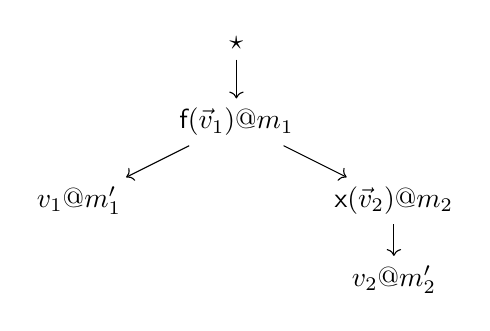
\begin{tikzpicture}
    \graph [no placement]
    {
      "$\star$" [at={(0,1)}] ->
      "$\mcall{f}{\vec{v}_1}{m_1}$" -> {
        "$\mret{v_1}{m_1'}$" [at={(-2,-1)}],
        "$\mcall{x}{\vec{v}_2}{m_2}$" [at={(+2,-1)}] ->
        "$\mret{v_2}{m_2'}$" [at={(+2,-2)}]
      }
    };
  \end{tikzpicture}
\end{center}
The initial move is a function call into the module,
which can perform
an arbitrary number of external calls
before answering the initial function call
with its own return move.
For example, a possible interaction is:
\[
  \mcall{f}{}{m_1}\ph{f} \ \cdot\ 
  \pt{f}
    \pcall{x}{1}{m_2}\ph{x} \ \cdot\ 
    \pt{x}\mret{7}{m_3} \ \cdot \ 
  \pt{f}
    \pcall{y}{22}{m_4}\ph{y} \ \cdot\ 
    \pt{y}\mret{5}{m_5} \ \cdot\ 
  \pt{f}\pret{0}{m_6}
\]
By convention,
in examples we name $f, g, h$
the functions exported by the module being considered,
and we name $x, y, z$
any external functions.
Moreover,
the polarity of moves makes it easy to distiguish
between the two versions of $\mcall{f}{\vec{v}}{m}$
and $\mret{v}{m'}$.

[Note the correspondance with Princeton core semantics.]

Note that once [an external function has been called
it might return more than once,
and more generally context can be non-innocent].

%}}}

\paragraph{General pattern} %{{{

Next we must the determine how to associate a strategy for $!\EC \multimap \EC$
to a given program $p$.
%for an interaction prefix $\mathbf{u} \in P_{!\EC \multimap \EC}$,
%we need to determine the next move of the program.
The construction follows a general pattern.
For a given language we define:
\begin{itemize}
  \item a set of states $s \in S$;
  \item a transition relation $[s \Rightarrow s']$;
  \item a predicate $I[s, f(\vec{v})@m]$,
    asserting that the state $s$ is an initial state
    corresponding to a call to the function $f$
    with arguments $\vec{v}$
    in an initial memory state $m$;
  \item a predicate $E[s, \pcall{x}{\vec{v}}{m}]$,
    asserting that state $s$
    corresponds to an external call to function $x$,
    with arguments $\vec{v}$
    in a memory state $m$;
  \item a predicate $R[s, \mret{v}{m}, s']$,
    which asserts that updating the state $s$
    to take into account the outcome $v@m$
    of an external call it performs
    will yield the new state $s'$;
  \item a predicate $F[s, \pret{v}{m}]$,
    which asserts that $s$
    is a final state
    returning the value $v$
    with a final memory state $m$.
\end{itemize}
This set of data
essentially constitute a big-step version of
the \emph{interaction semantics} used in \citep{compcompcert}.
They are used to build a new transition system
over $S \times P_{!\EC \multimap \EC}$
where states are instrumented with a log of the interaction:
\begin{gather*}
  \AxiomC{$[s \Rightarrow s']$}
  \UnaryInfC{$(s, \mathbf{u}) \rightarrow (s', \mathbf{u})$}
  \DisplayProof
  \\
  \AxiomC{\rule{0pt}{1.5em}$E[s, \pcall{x}{\vec{v}}{m}]$}
  \UnaryInfC{$
    (s, \mcall{f}{\vec{v}_0}{m_0}       \cdot \mathbf{u})
    \rightarrow
    (s, \mcall{f}{\vec{v}_0}{m_0}\ph{f} \cdot \mathbf{u} \cdot
        \pt{f} \pcall{x}{\vec{v}}{m})$}
  \DisplayProof
  \\
  \AxiomC{\rule{0pt}{1.5em}$R[s, \mret{v}{m}, s']$}
  \UnaryInfC{$
    (s,  \mcall{f}{\vec{v}_0}{m_0}\ph{f} \cdot \mathbf{u} \cdot
         \pt{f}\pcall{x}{\vec{v}}{m})
    \rightarrow
    (s', \mcall{f}{\vec{v}_0}{m_0}\ph{f} \cdot \mathbf{u} \cdot
         \pt{f}\pcall{x}{\vec{v}}{m}\ph{x} \cdot
         \pt{x}\mret{v}{m'})$}
  \DisplayProof
  \\
  \AxiomC{\rule{0pt}{1.5em}$F[s, \pret{v}{m}]$}
  \UnaryInfC{$
    (s,  \mcall{f}{\vec{v}_0}{m_0} \cdot \mathbf{u})
    \rightarrow
    (*, \mcall{f}{\vec{v}_0}{m_0}\ph{f} \cdot \mathbf{u} \cdot
        \pt{f}\pret{v}{m})$}
  \DisplayProof
\end{gather*}
Then the corresponding strategy $\sigma : {!\EC} \multimap \EC$
can be defined as:
\[
  \sigma =
    \{ \mathbf{u} \: | \:
       \exists \, s \, s' \,. \, I[s, \mcall{f}{\vec{v}}{m}] \wedge
       (s, \mcall{f}{\vec{v}}{m}) \rightarrow^* (s', \mathbf{u}) \}
\]
[XXX P-view needs to be involved
so that our strategy can handle ill-bracketed environments]
[Expliquer comment construire $e$ et quelles sont
les conditions sur nos pr\'edicats.]
[Omit pointers and polarities for clarity and mention that
since we're working over $P_{!\EC \multimap \EC}$ it will be fine?]

This is similar to the approach taken in \citep{osdi16},
where the memory states are instrumented
with a log of the current interaction,
which is used by a fixed $\kw{external\_call}$ predicate
to query an oracle representing the environment.
In the context of our strategies,
we do not need an oracle
but instead non-deterministically explore
all possible behaviors for the environment.
Moreover,
the log and external calls reside
outside of the original small-step semantics,
so that we simply pass an empty $\kw{external\_call}$ predicate to it
and do not need to instrument memory states it uses.

%}}}

\paragraph{Semantics of Clight} %{{{

To compute the semantics $\kw{ClightX}(p) : \: !\EC \multimap \EC$
we define $S$ to be the set of Clight states.
The definition of the predicates is:
\begin{align*}
  [s \Rightarrow s'] &\Leftrightarrow
    \kw{ClightX}_\bot(p) : s \rightarrow^* s' \\
  I[s, \mcall{f}{\vec{v}}{m}] &\Leftrightarrow
    s = \kw{CallState}(f, \vec{v}, m, \kw{Kstop}) \\
  E[s, \pcall{x}{\vec{v}}{m}] &\Leftrightarrow
    s = \kw{CallState}(x, \vec{v}, m, k) \\
  R[s, \mret{v}{m'}, s'] &\Leftrightarrow
    s = \kw{CallState}(x, \vec{v}, m, k) \wedge
    s' = \kw{ReturnState}(v, m', k) \\
  F[s, \pret{v}{m'}] &\Leftrightarrow
    s = \kw{ReturnState}(v, m', \kw{Kstop})
\end{align*}

%}}}

\paragraph{Semantics of Asm} %{{{

The semantics of Asm is less straightforward to define,
because we have to take into account the C calling convention
when considering the memory states and argument values
that constitute the interaction with the environment.

[TBD, we can try to define a C-style semantics of Asm,
or introduce a new game for Asm interaction.]

%}}}

Note that the more limited semantics of the previous section
may be obtained by:
\[ \kw{ClightX}_\mathcal{E}(p) \equiv_\kw{id} \kw{ClightX}(p) \circ \mathcal{E}^\dagger \]

%}}}

\subsection{Semantic linking} %{{{

While ${!\EC} \multimap \EC$ is sufficient
to interpret the semantics of Compcert programs,
the work presented here goes one step further
and uses strategies for ${!\EC} \multimap {!\EC}$
as its semantic domain.
In that game,
when a module calls back into the environment,
instead of returning immediately
the environment itself
can perform a nested call into the module,
and so on recursively.
In the case of a Compcert program,
the nested function calls behave uniformly,
and we can simply run a second copy of
the corresponding strategy,
through the use of the $-^\dagger$ operator.
However,
our semantics domain is richer
and allows strategies with hidden state
and control effects
not present in Compcert languages.

A possible interaction in ${!\EC} \multimap {!\EC}$ is:
\[
  \rule{0pt}{1.5em}
  \mcall{f}{}{m_1}\ph{f} \ \cdot\ 
  \pt{f}
    \pcall{x}{1}{m_2}\ph{x} \ \cdot\ 
    \pt{x}
      \mret{7}{m_3} \ \cdot \ 
  \pt{f}
    \pcall{y}{22}{m_4}\ph{y} \ \cdot\ 
      \mcall{g}{}{m_5}\ph{g} \ \cdot\ 
      \pt{g}\pret{1}{m_6} \ \cdot\ 
    \pt{y}
      \mret{5}{m_7} \ \cdot\ 
  \pt{f}\pret{0}{m_8}
\]
First,
the function $f$ implemented by the module
is called with no arguments
and with an initial memory $m_1$.
$f$ performs two external calls:
first to $x$, which returns immediately,
then to $y$.
In its turn,
the external function $y$ calls
the function $g$, which is also implemented by the module.
after $g$ returns $1$ to $y$,
then $y$ returns $5$ to $f$,
which finally returns $0$ to the environment
as the answer to the initial question.

{ \color{gray}
\paragraph{Views}

The \kw{P}-view
gives a trace of all external calls executed so far
\emph{in the context of the current activation frame}.
Consider the prefix of the example above
obtained by dropping the last move.
The \kw{P}-view is:
\[
  \rule{0pt}{1.5em}
  \mcall{f}{}{m_1}\ph{f} \ \cdot\ 
  \pt{f}
    \pcall{x}{1}{m_2}\ph{x} \ \cdot\ 
    \pt{x}
      \mret{7}{m_3} \ \cdot \ 
  \pt{f}
    \pcall{y}{22}{m_4}\ph{y} \ \cdot\ 
    \pt{y}
      \mret{5}{m_7}
\]
Intuitively,
a given activation of $f$
only sees its \emph{immediate} interaction with the environment
(namely, the calls to $x$ and $y$ as well as their ultimate outcomes),
but the call back to $g$ performed by $y$,
as well as any further interaction that could have occured
during the execution of $g$,
are removed from its view.
An innocent strategy will not be permitted to
depend on these intermediate events
to determine what will come next in the execution of $f$.
While this may seem restrictive,
especially for a stateful language such as C,
remember that our move carry the global memory state,
so that any changes made by $g$ in $m_6$
will presumably be reflected in the memory state $m_7$
passed back to $f$ along with $x$'s return value.
Innocence therefore simply states that
any state kept by the module is explicit and passed back
through the environment.
}

%he \kw{O}-view is:
%[
% \rule{0pt}{1.5em}
% \mcall{f}{}{m_1}\ph{f} \ \cdot\ 
% \pt{f}
%   \pcall{y}{22}{m_4}\ph{y} \ \cdot\ 
%     \mcall{g}{}{m_5}\ph{g} \ \cdot\ 
%     \pt{g}\pret{1}{m_6} \ \cdot\ 
%   \pt{y}
%     \mret{5}{m_7} \ \cdot\ 
%]

Now consider the strategies
$\sigma_1, \ldots, \sigma_n : {!\EC} \multimap {!\EC}$,
and assume they provide behaviors
for the respective sets of function names $F_1, \ldots, F_n$.
We want to define
a combined strategy $\mathcal{L}_F(\sigma_1, \ldots \sigma_n)$
which will provide behaviors for
all of the functions in $F = F_1 \cup \cdots \cup F_n$,
where any call back to $f \in F$ by any of linked strategies
is handled by an interaction among them.
Note that this interaction
can potentially be mutually recursive.

The first step is to construct the union
$\sigma = \sigma_1 \cup \cdots \cup \sigma_n$.
The strategy $\sigma$
contains all of the ``flat'' behaviors of the $\sigma_i$'s,
however at this point
external calls performed by any of the individual strategies
are still directed to the environment
whether or not the target function is in $F$.

To discriminate between external and mutual calls,
we introduce the primitive $\lhd_F : {!\EC} \otimes {!\EC} \multimap \EC$.
The idea is that $\lhd_F(\mathcal{E}_1, \mathcal{E}_2) : \EC$
will use $\mathcal{E}_1$ to handle calls to any $f \in F$,
and use $\mathcal{E}_2$ to handle calls to any $g \notin F$.
Formally:
\begin{definition}[$\lhd_F$]
For a given set of identifiers $F : \mathcal{P}(\kw{ident})$,
$\lhd_F : {!\EC} \otimes {!\EC} \multimap \EC$ is the strategy defined by
the prefix closure of:
\begin{align*}
  \lhd_F &\ni
    \mcall{f}{\vec{v}}{m}\ph{f} \cdot
    \pt{f}\underline{i_1(\mcall{f}{\vec{v}}{m})}\ph{f1} \cdot
    \pt{f1}i_1(\mret{v}{m'}) \cdot
    \pt{f}\pret{v}{m'}
    \quad (f \in F) \\
  \lhd_F &\ni
    \mcall{x}{\vec{v}}{m}\ph{x} \cdot
    \pt{x}\underline{i_2(\mcall{x}{\vec{v}}{m})}\ph{x2} \cdot
    \pt{x2}i_2(\mret{v}{m'}) \cdot
    \pt{x}\pret{v}{m'}
    \quad (x \notin F)
\end{align*}
\end{definition}

The linked strategy will be obtained by taking a fixed point,
so that whenever $\sigma$ calls back into one of the linked modules,
this call is directed to another copy of $\sigma$,
and so on to an arbitrary depth.
Schematically:
\begin{center}
  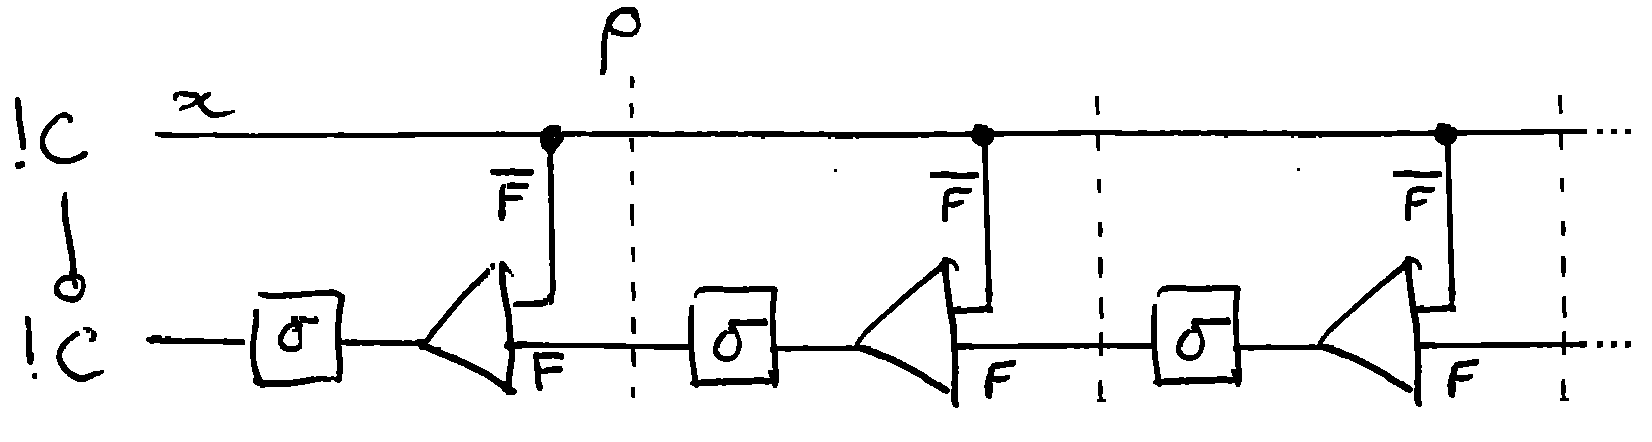
\includegraphics[scale=0.7]{linking-operator}
\end{center}
This can be described informally as:
\[
  \mathcal{L}_F(\sigma) \approx
  \mu \rho . \lambda x . \sigma (\lhd_F (\rho x, x))
  : {!\EC} \multimap {!\EC}
\]
In the above,
$x : {!\EC}$ represents the domain of $\mathcal{L}_F(\sigma)$,
towards which we can direct $\sigma$'s truly external calls,
whereas $\rho : {!\EC} \multimap {!\EC}$ is a ``recursive copy'' of $\mathcal{L}_F(\sigma)$,
which we can use to handle the internal calls emitted by $\sigma$
so long as we provide a copy of $x$
for $\rho$ to use for its own external calls.

Similarly to the interpretation of recursion
in the game semantics of PCF,
we can construct the least fixed point $Y(f) : A$
of a strategy $f : A \multimap A$
as the upper bound:
\[
  Y(f) = \bigcup_{k=0}^\infty f_k\,,
\]
where $f_0 = \bot_{A}$ is the empty strategy
and $f_{k+1} = f(f_k)$.
The sequence is increasing:
$\bot \subseteq f(\bot)$,
and by monotony of application,
if $f_k \subseteq f_{k+1}$,
then $f_{k+1} = f(f_k) \subseteq f(f_{k+1}) = f_{k+2}$.

It remains to describe a strategy
$\tilde{\sigma} : ({!\EC} \multimap {!\EC}) \multimap ({!\EC} \multimap {!\EC})$
whose fixed point is the strategy we want.
We can formalize the description above
in the context of the symmetric monoidal close category $\mathcal{G}$
as follows:
\[
  \tilde{\sigma} =
    \Lambda
      \left(
      \sigma \circ
      \lhd_F^\dagger \circ
      (\kw{eval}_{{!\EC}, {!\EC}} \otimes \kw{id}_{!\EC}) \circ
      (\kw{id}_{{!\EC} \multimap {!\EC}} \otimes \Delta_\EC^\dagger)
      \right)
\]
The inner term,
of type $({!\EC} \multimap {!\EC}) \otimes {!\EC} \multimap {!\EC}$,
can be visualized as:
\begin{center}
  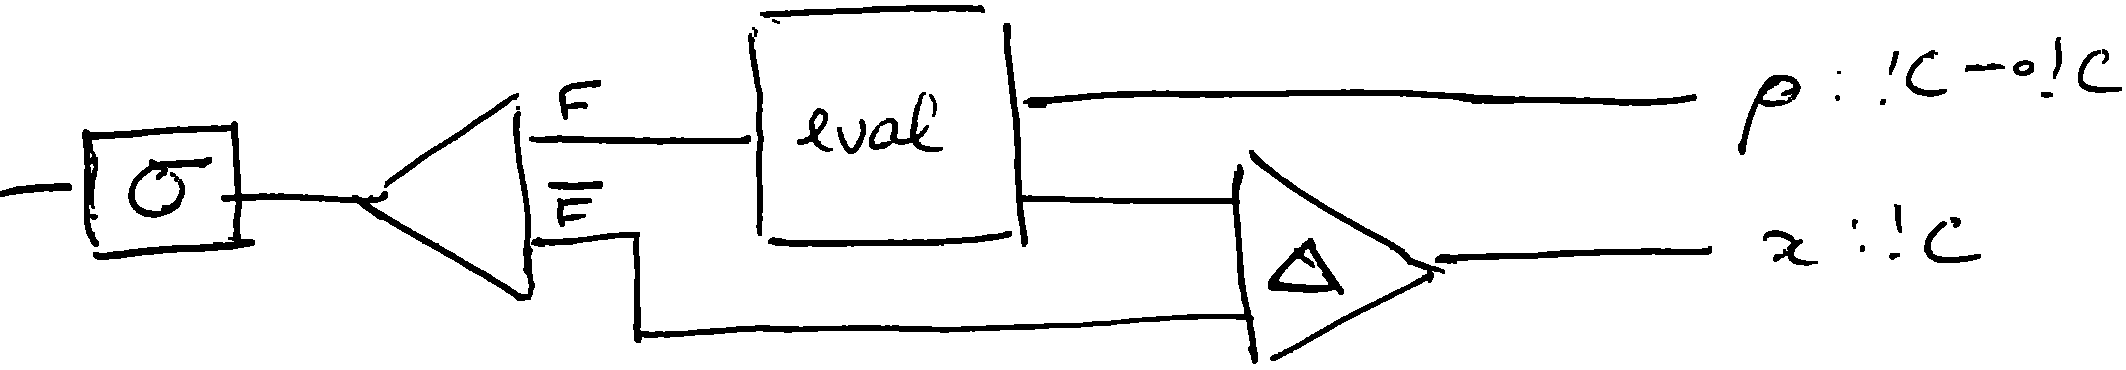
\includegraphics[scale=0.6]{linking-element}
\end{center}
We can finally define:
\[
  \mathcal{L}_F(\sigma_1, \ldots, \sigma_n) = \kw{Y}(\tilde{\sigma})
\]

%}}}

\subsection{External functions [?]} %{{{

[By which I mean the semantics of external functions
including memcpy, malloc, free \ldots
The semantics of those can be defined as strategies
and linked back.]

[One issue is:
Compcert's correctness theorem is
assuming that external functions behave in a certain way.
So if we remove them completely into an oracle
it won't be valid any more.
But,
we'd like to get rid of events completely,
so it'd ...]

%}}}

\subsection{Relations} %{{{

[Move to next section?]

A \emph{Kripke logical relation between games} $A$ and $B$
is a Kripke logical relation $R : \mathcal{R}_W(M_A, M_B)$
between the possible moves of $A$ and $B$
such that:
\begin{gather*}
  (\star \vdash_A) \ifr{\Diamond R \rightarrow (\Rightarrow)} (\star \vdash_B) \\
  (\vdash_A) \ifr{\Box(R \rightarrow \Diamond R \rightarrow (\Rightarrow))} (\vdash_B) \\
  \lambda_A \ifr{\Box (R \rightarrow (=))} \lambda_B \\
  R^\oast(P_A) \subseteq P_B
\end{gather*}
We write $R : \mathcal{R}_W(A, B)$.


[XXX polarity for $\vdash$: you want to relate environment moves
in the other direction]
[XXX we need te environment half of the simulation
in the game relation, not just even the guarantee that it would yield
legal moves]
[XXX note for KLR section: picking between
the different relations at some type is arbitrary choice,
in effect those are different structures
but their ``flattened'' interpretations in terms of sets are identical.
For instance compare $R \rightarrow R \rightarrow \Rightarrow$
(order-preserving relation)
with $R \rightarrow \mathcal{P}^+(R)$
(simulation relation)
in the first case we look at $\langle A, \rightarrow \rangle$
as potentially some kind of order relation,
in the second case we look at $\langle A, \rightarrow \rangle$
as a transition system.]

From logical relation of arenas, relation on positions.
Explain KLR aspect also.

%}}}

%}}}

\section{Compositional correctness of CompCertX} %{{{

Recall the correctness theorem of CompCertX:
\[
  \begin{tikzcd}[column sep=large]
    \mcall{f}{\vec{v}}{m}
      \arrow[r, "\kw{Clight}(p)"]
      \arrow[d, dash, "="'] &
    \mret{v}{m'}
      \arrow[d, hookrightarrow, "\iota'"] \\
    \mcall{f}{\vec{v}}{m}
      \arrow[r, dotted, "\kw{Asm}(\mathcal{C}(p))"'] &
    \mret{v'}{m''}
  \end{tikzcd}
\]
The injection $\iota$
extends $\kw{flat\_inj}(\kw{nextblock}(m))$.
We can use the parametricity of $\kw{Asm}$
to obtain the more typical diagram:
\[
  \begin{tikzcd}[column sep=large]
    \mcall{f}{\vec{v}}{m}
      \arrow[r, "\kw{Clight}(p)"]
      \arrow[d, dash, "="'] &
    \mret{v}{m'}
      \arrow[d, hookrightarrow, "\iota'"] \\
    \mcall{f}{\vec{v}}{m}
      \arrow[r, dotted, "\kw{Asm}(\mathcal{C}(p))"']
      \arrow[d, hookrightarrow, two heads, "\iota"'] &
    \mret{v'}{m''}
      \arrow[d, hookrightarrow, two heads, "\iota''"] \\
    \mcall{f}{\vec{v}_2}{m_2}
      \arrow[r, dotted, "\kw{Asm}(\mathcal{C}(p))"'] &
    \mret{v'}{m''}
  \end{tikzcd}
\]

Compositional CompCert:
\begin{quote}
A deficiency of CompCert's simulation proofs and of LSRs
was that they assumed conditions (1) and (2) at external calls,
but did not prove that these properties were preserved by compilation.
Directly imposing constraints (1) and (2)
onto the simulation clauses for internal steps does not work, however.
A compiled function should be allowed to
write to its own spill locations ---
just not to those of its caller.
\end{quote}
Goes on to define massively complicated \emph{structured injections}.

But we don't need to!
Our KLR framework
mapped onto justification pointers
expresses just the right constraints!

%}}}

\section{Linking with fancy contexts} %{{{

Show that we can link soundly with thread library, longjmp, cswitch, etc.

Verify some mixed C/asm program that uses this kind of assembly primitives.

\subsection{Long jumps}
\label{sec:longjmp}

The C standard library provides the following primitives
which implement ``non-local jumps'':
\begin{description}
\item[\texttt{setjmp(jmp\_buf env)}]
    saves the stack context into \texttt{env}
    and returns ...
\item[\texttt{longjmp(jmp\_buf env)}]
    interrupts normal control flow
    and restores the stack context previously saved in \texttt{env},
    causing the corresponding call to \texttt{setjmp}
    to return again,
    this time a non-zero value.
\end{description}
Because \kw{longjmp} triggers a control effect,
its semantics cannot be described
as that of a classical Compcert external function call.
However,
a version of \kw{setjmp} and \kw{longjmp}
can be modelled naturally as the strategy $\sigma_\kw{jmp}$
defined by the prefix closure of the following language:
\[
    \small
    \left(
    (\texttt{setjmp}()@m_i\ph{p1}\ \cdot\ \pt{p1}\underline{0@m_i})^* \ \cdot\ 
    \texttt{setjmp}()@m\ph{p} \ \cdot\ \pt{p}\underline{0@m}\ \cdot\ 
    \texttt{longjmp}()@m'\ \cdot\ \pt{p}\underline{1@m'}
    \right)^*
\]

Interesting to consider what happens in
oracle-based oracle semantics and simulation proof.

%}}}

\section{Related Work} %{{{

Interaction semantics is an automaton formulation of $EC \Rightarrow EC$
(follows Ghica 2012),
but our semantic domain more open-ended and
we can use Compcert with fancier games
(say event traces etc).
Also,
by oversimplifying they've given up the structure
that allows us to define our magical KLRs
and they have to put it back in,
in a much more contrived and ad-hoc way.
(Also by mixing internal steps and interaction steps per Ghica 2012.)

%}}}

\section{Future work} %{{{

Simulation among different games,
also $\sigma^+ \le \tau^+$.

%}}}

%}}}

\end{document}
